\documentclass[a4paper,12pt]{report}

\usepackage[margin=2.5cm, inner=4cm, outer=2cm]{geometry}
\usepackage[T1]{fontenc}
\usepackage[utf8]{inputenc}
\usepackage{lmodern}
\usepackage{graphicx}
\usepackage{textcomp}
\usepackage{fancyvrb}
\usepackage[german]{babel}
\usepackage{framed}
\usepackage{setspace}
\usepackage{hyperref}

\onehalfspacing
\setcounter{tocdepth}{3}
\setcounter{secnumdepth}{3}

\addto\captionsgerman{\renewcommand{\chaptername}{Teil}}

\title{{Funktionsweise eines Raycasters mithilfe eines selber geschriebenen Beispiels erkl\"art \vspace{1cm}} \\
        {\large Informatik GK1, Herr Berger} \\
        {
\includegraphics[width=10cm]{sge.jpg}}}
\author{Andreas Gwilt}

\newcommand{\mychapter}[2]{
    \setcounter{chapter}{#1}
    \setcounter{section}{0}
    \chapter*{#2}
    \addcontentsline{toc}{chapter}{#2}
}

\begin{document}

\maketitle
\tableofcontents

\setcounter{page}{0}

\mychapter{1}{Einleitung}

\section{Was ist ein Raycaster?}
Ein Raycaster ist eine Rendermethode, die eine pseudo-3D Welt basierend auf einem 2D Spielfeld rendert\cite{scratch}.

Raycasting ist eigentlich ein ziemlich weiter Begriff, der meistens f\"ur die Rendermethode benutzt wird. Allgemein ist es aber eine Technik, um zu sehen, ob ein Strahl einen K\"orper schneidet. Man ``wirft'' einen Strahl, und \"uberpr\"uft, ob er eine Ebene schneidet oder nicht. Diese ist dem Raytracing sehr \"ahnlich, aber ist viel limitierter und auch schneller. Im Gegensatz zu Raycasting (was f\"ur jeden Pixel oder jede Spalte von Pixeln des Bildschirms einen Strahl wirft) simuliert Raytracing ann\"ahernd die Photonen, die von Lichtquellen auf Ebenen reflektieren und eventuell das Auge erreichen.

Ich habe, um den Raycaster zu erkl\"aren, eine in der ersten Person gerenderten Version von Conways \textit{Spiel des Lebens}\cite{life} geschrieben, die einen Raycaster zum Rendern benutzt. In dieser Facharbeit werde ich die Funktionsweise des Raycasters erkl\"aren.

\begin{figure}[htbp] 
        \centering
        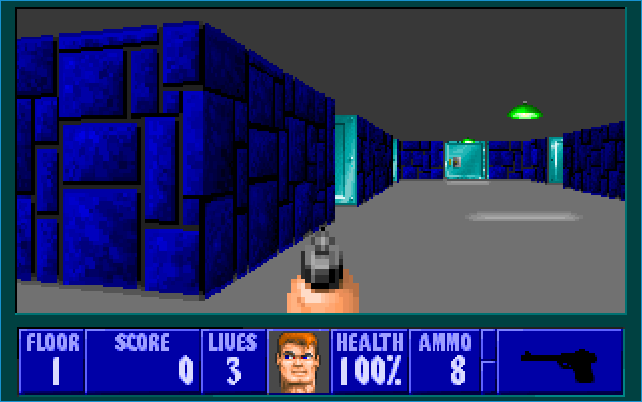
\includegraphics[width=4in]{wolf3d.png} 
        \caption{Wolfenstein 3D, ein Spiel, das einen Raycaster verwendete.}
        \label{fig:wolf3d}
\end{figure}

\section{Welche Probleme l\"ost ein Raycaster?}
Raycasting ist eine Methode, um zu \"uberpr\"ufen, ob ein Strahl eine Fl\"ache schneidet oder nicht. Die h\"aufigste Anwendung daf\"ur ist als einfaches Renderverfahren, um ein Spielfeld in Pseudo-3D darzustellen. Es gibt aber auch mehrere andere Anwendungen, z.B. Kollisionserkennung oder um fest zu stellen, ob etwas von einem Punkt aus sichtbar ist oder nicht.

\paragraph*{}
In den fr\"uhen 1990ern, als Raycasting beliebt wurde, hatte man noch ziemlich wenig Rechenleistung, wollte aber ``3D'' Spiele schreiben. Eine wirklich dreidimensionales Spiel-Engine (wie die 1996 erschienene Quake Engine) war noch nicht schnell genug, um in einem Spiel benutzt zu werden, also verwendete man Methoden wie Raycasting, um die Illusion von 3D herzustellen. Das vielleicht ber\"uhmteste Spiel, was Raycasting benutzte, war Wolfenstein 3D (Auch der erste beliebte Ego-Shooter). Wolfenstein 3D hatte ein zweidimensionales Spielfeld, was in 3D dargestellt wurde.

Raycasting musste jedoch sehr viele Kompromisse eingehen, um so schnell zu sein. Das Spielfeld war ein zweidimensionales Array, also konnte es nur Rechte Winkel geben, und Decke und Boden mussten immer gleich hoch bleiben. Man erkennt an Abb~\ref{fig:wolf3d} deutlich, dass das Spiel nicht wirklich dreidimensional ist. Auch sieht das Bild blockhaft aus, und die Beleuchtung ist nicht realistisch.

\section{Die Geschichte des Raycasters}
Raycasting wurde schon diskutiert, lange bevor PCs leistungsstark genug waren, um es wirklich in Spielen zu benutzen. Eine 1982 ver\"offentlichte Abhandlung von Scott Roth beschreibt Raycasting als Methode, dreidimensionale K\"orper zu rendern.

Eines der ersten Spiele, die das Prinzip implementierten, war \textit{Hovertank 3D}, was in April 1991 von id Software ver\"offentlicht wurde. \textit{Hovertank 3D} war noch sehr primitiv und hatte noch keine Texturen auf den W\"anden, aber es war der Anfang eines neuen Genre von Spielen. Im darauffolgenden November erschien \textit{Catacomb 3-D}, was Texturen hatte, und oft als der erste Ego-Shooter gesehen wird.

Zufrieden mit den zwei ``Prototypen'' entwickelten id Software ein neues Spiel:\\
\textit{Wolfenstein 3D}, was 1992 ver\"offentlicht wurde, war ein gro\ss er Erfolg und machte Ego-Shooter, und damit den Raycaster, bekannt.

Heutzutage findet der Raycaster nicht mehr viel Verwendung als Renderer, aber das Prinzip wird mit dem Raytracer fortgef\"uhrt. Der Raytracer arbeitet immer in drei Dimensionen, und ist rekursiv, d.h. er simuliert den kompletten Gang eines Lichtstrahles, inklusiv Reflexionen. Raytracing ist aber noch immer zu langsam f\"ur Echtzeit Darstellung, und findet eher als Renderer von stillen Bildern Gebrauch.


\mychapter{2}{Wie funktioniert ein Raycaster?}
\section{Allgemein}

\subsection{Was macht ein Raycaster?}
Allgemein gesehen muss ein Raycaster den ersten Schnittpunkt zwischen einem Strahl (theoretisch eine Halbgerade) und einem K\"orper finden. Wir stellen uns vor, dass ein Strahl von einem Punkt (das Auge des Spieler) aus in einer bestimmten Richtung verl\"auft. Wir f\"uhren diesen Strahl immer weiter, bis er auf etwas trifft. Dann berechnen wir die L\"ange des Strahls, und wissen wie weit das Objekt weg ist. Man kann das in beliebig vielen Dimensionen machen, aber der Raycaster ist zweidimensional.

F\"ur jede Spalte des Fensters/Bildschirms wirft er einen Strahl (also z.B. 1920 Strahlen bei einer FHD Aufl\"osung), und sieht wie weit weg er auf etwas st\"o\ss t. Entsprechend wird dann eine vertikale Linie auf dem Bildschirm gemalt. Abb~\ref{fig:rcaster} zeigt ein Diagramm dazu.
\begin{figure}[htbp] 
        \centering
        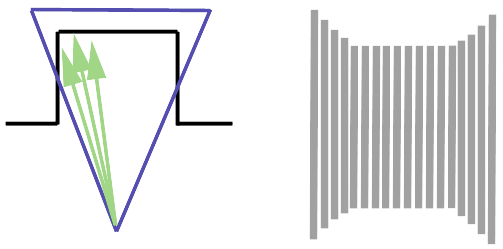
\includegraphics[width=8cm]{raycasting.png} 
        \caption{Bild von \url{http://www.fabiensanglard.net/wolf3d/index.php}}
        \label{fig:rcaster}
\end{figure}

Leider ist es aber sehr langsam, f\"ur jeden Pixel des Strahls zu sehen, ob er in einem Objekt oder nicht ist. Deshalb sehen wir das Spielfeld als Gitter (Siehe Abb.~\ref{fig:grid}), und m\"ussen so an viel weniger Stellen pr\"ufen. In dem Gitter ist der Spieler P in dem Feld (0,3). Der Strahl (der von P kommt und den Winkel $\alpha$ hat) muss jetzt nur an dem ersten Punkten in (1,3), (1,2), (2,2) und (2,1) gepr\"uft werden.
\begin{figure}[htbp]
        \centering
        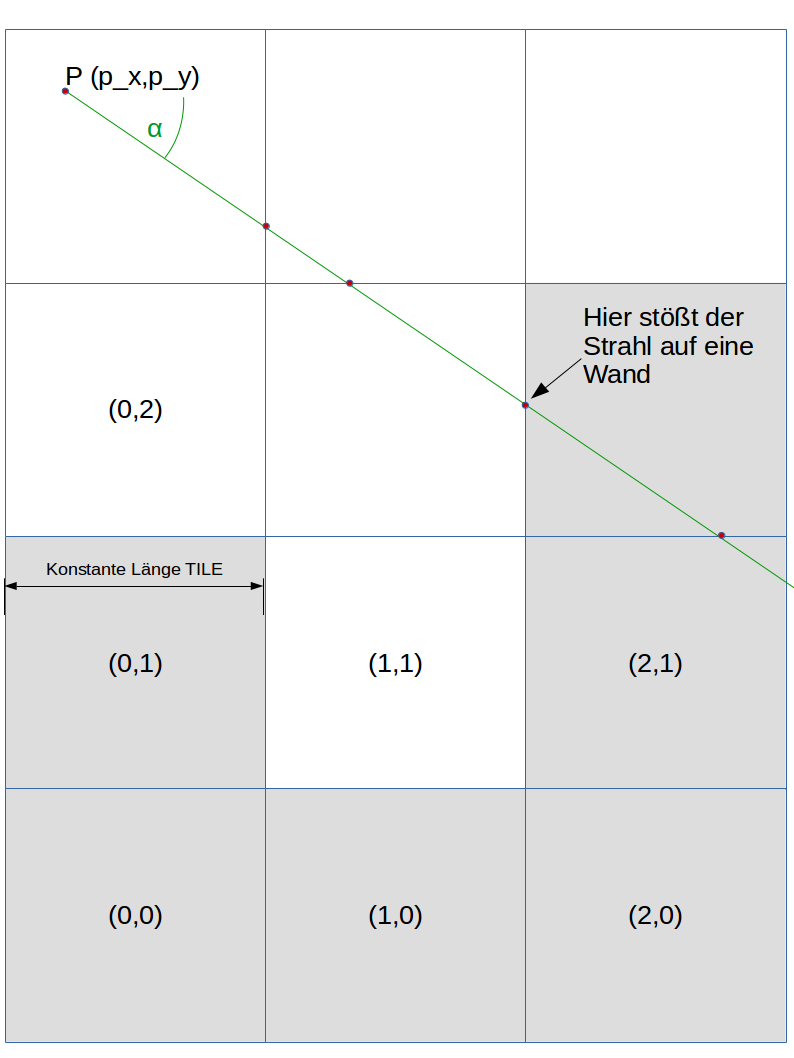
\includegraphics[width=8cm]{grid.png} 
        \caption{An den roten Punkten geht der Strahl in ein neues Feld}
        \label{fig:grid}
\end{figure}

Bevor wir weiter gehen, ist es wichtig zu wissen, welche Variablen existieren, und wie sie hier hei\ss en.

\subsection{Daten}
\subsubsection{Koordinaten}
Weil wir das Spielfeld jetzt als Gitter sehen, haben wir auch zwei verschiedene Typen von Koordinaten: ``normale'' Koordinaten, z.B. wo der Spieler steht, und \texttt{world}- oder Gitterkoordinaten, die gr\"oberen Koordinaten des Spielfeldes.

Das Spielfeld ist n\"amlich ein zweidimensionales Array, das 1 (f\"ur eine Wand) oder 0 (f\"ur leeren Raum) enth\"alt. Dieses Modell ist nat\"urlich erweiterbar: Man k\"onnte auch Zahlencodes f\"ur Texturen oder einfach Farben in der Array haben. Als Beispiel eine Array, die das Spielfeld in Abb.~\ref{fig:grid} speichert:
\begin{Verbatim}[baselinestretch=1.0, xleftmargin=1cm]
world = [[1,1,0,0],
         [1,0,0,0],
         [1,1,1,0]]
\end{Verbatim}
Um z.B. Feld (0,1) zu finden, sehen wir einfach in \texttt{world[0][1]} nach. F\"ur die Breite und H\"ohe des Spielfeldes sind \texttt{hl} (Horizontale L\"ange) und \texttt{vl} zust\"andig. 
\paragraph*{}
F\"ur den Spieler, den Strahl, und eventuellen Gegnern wollen wir aber genauere Koordinaten haben. Dazu m\"ussen wir wir definieren, wie lang ein \texttt{world}-Feld in den genauen Koordinaten ist. Die Gr\"o\ss e nenne ich \texttt{TILE} (in diesem Fall auf 32 gesetzt).

Der Spieler hat die genauen Koordinaten \texttt{p\_x} und \texttt{p\_y}, und den Winkel \texttt{p\_a}. Um die \texttt{world}-Koordinaten des Spielers zu finden, teilen wir ohne Rest durch die L\"ange eines Feldes, z.B. \texttt{world[p\_x // TILE][p\_y // 64]}. Das bringt uns zu noch einem wichtigem Punkt:

\subsubsection{Winkel}
Alle Winkel in meinem Programm sind im Bogenma\ss , und zeigen ``nach unten'' von der Horizontalen (Abb.~\ref{fig:angles}). Auch gehen alle Funktionen davon aus, dass ein Winkel immer positiv und immer unter $2\pi$ bleibt.
\begin{figure}[htbp] 
        \centering
        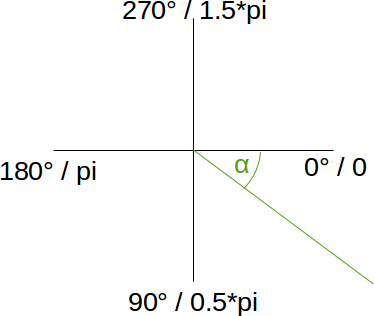
\includegraphics[width=4cm]{angles.png} 
        \label{fig:angles}
\end{figure}

\subsubsection{Liste}
In dem Anhang steht eine Liste der wichtigen Variablen, mit datantyp:


\subsection{Was macht ein Raycaster -- genauer}
Wenn man die Punkte in Abb~\ref{fig:grid} noch einmal betrachtet, f\"allt auf, dass eine H\"alfte auf den vertikalen, und die andere auf den horizontalen ist. Es macht Sinn, beide separat zu \"uberpr\"ufen, weil man dann mit einem konstanten Wert inkrementieren kann.

Betrachten wir die vertikalen Schnittstellen: alle sind auf der x-Achse eine Feldl\"ange (\texttt{TILE}) entfernt. Auch auf der y-Achse sind sie in einem konstanten Intervall voneinander entfernt. F\"ur die horizontalen ist es gleich, nur x und y sind vertauscht. Zur\"uck zu den vertikalen Schnittstellen.

Wenn wir den ersten Punkt gefunden haben, wo der Strahl eine vertikale Grenze des Gitters \"uberschreitet, pr\"ufen wir nach, ob dieser Punkt in \texttt{world}-Koordinaten gef\"ullt (1) oder nicht (0) ist. Wenn nicht, erweitern wir den Strahl, indem wir zu unserem ersten Punkt die Intervalle \texttt{x\_i} und \texttt{y\_i} addieren. Das wird wiederholt, bis der Strahl auf etwas trifft (also in einem \texttt{1} Feld steht).

Das gleiche wird dann noch mal mit den horizontalen Schnittstellen gemacht, bis man zwei Punkte oder Distanzen (zu den Punkten) hat. Dann kann die k\"urzere Distanz zur\"uckgegeben werden, und f\"ur das Rendern oder Gehen benutzt werden.

\section{Schritt f\"ur Schritt Erkl\"arung}

.. oder ``Was macht ein Raycaster -- noch viel genauer''. Hier wird die Vorgehensweise und der Code Schritt f\"ur Schritt erkl\"art, beginnend bei der Initialisierung diverser Variablen.

\subsection{Initialisierung}

Zuerst m\"ussen einige Variablen gesetzt werden. Einige werden in dem ganzen Spiel konstant bleiben:
\begin{Verbatim}[baselinestretch=1.0, xleftmargin=1cm]
TILE = 32 # L\"ange der Ziegel von world
pi = math.pi

plane_x = 1280 # Bildschirm/Fenster Aufl\"osung
plane_y = 720
fov = math.radians(60) # Sichtfeld
\end{Verbatim}

Jetzt kommen einige Variablen f\"ur das Spielfeld und den Spieler, die zum Teil ge\"andert werden k\"onnen (z.B. Spielerposition):
\begin{Verbatim}[baselinestretch=1.0, xleftmargin=1cm]
hl = 100 # Horizontale/vertikale L\"ange des Spielfeldes
vl = 50
world = [[0 for i in range(vl)] for j in range(hl)] # Welt array
p_x = 32 # Spieler x,y
p_y = 32
p_a = 0 # Spieler Winkel (zeigt am Moment nach "rechts")

plane_d = (plane_x / 2) / math.tan(fov/2) # distance to plane
ray_angle = fov / plane_x # angle between rays
\end{Verbatim}

\subsection{Die zentrale Schleife / \texttt{draw} Funktion}
\subsubsection{Schleife}
Danach wird \texttt{pygame} (Die Graphik-Library) initialisiert, und die zentrale Schleife angefangen. Spiel-schleifen haben in der Regel drei Schritte:
\begin{enumerate}
	\item Befehle von dem Benutzer holen
	\item Mit dieser Information den Spielzustand erneuern
	\item Das Spiel rendern
\end{enumerate}
In meinem Beispiel ist Schritt 1. Nachschauen, welche Tasten gedr\"uckt werden. Entsprechend \"andert sich \texttt{p\_a}, wenn der Spieler sich drehen will, und \texttt{p\_x}/\texttt{p\_y}, wenn der Spieler sich bewegt. Dazu wird die \texttt{walk(world, p\_x, p\_y, a)} Funktion abgerufen, die mithilfe der \texttt{cast} Funktion pr\"uft, ob der Weg frei ist oder nicht. Danach wird das Spielfeld nach den \textit{Life}-Regeln von der \texttt{update(world)} Funktion aktualisiert.

\subsubsection{\texttt{draw()}}
Haupts\"achlich interessieren wir uns aber f\"ur die \texttt{draw(world)} Funktion, die das Ganze mithilfe des Raycasters rendert. Bevor das eigentliche Rendern anf\"angt, wird der Hintergrund gemalt. In diesem Fall hei\ss t das einfach, das Fenster wei\ss  zu f\"ullen, und f\"ur den Boden ein hellgraues Rechteck zu malen:
\begin{Verbatim}[baselinestretch=1.0, xleftmargin=1cm]
screen.fill((255,255,255))
pygame.draw.rect(screen, (200,200,200), \
((0,(plane_y/2)),(plane_x,plane_y)))
\end{Verbatim}

Wie beschrieben wirft man jetzt f\"ur jede Spalte des Fensters einen Strahl mit \texttt{cast}, und malt mit der Information einen Vertikalen Strich in der Spalte. Dazu muss man zuerst den Winkel des ersten Strahls finden. Dazu subtrahiert man die H\"alfte des Blickwinkels von dem Spieler-Winkel \texttt{p\_a}. Dabei muss man mod $2\pi$ bzw. 360\textdegree\ rechnen, damit man immer einen positiven Winkel hat.
\begin{Verbatim}[baselinestretch=1.0, xleftmargin=1cm]
angle = (p_a - (fov/2)) % (2*pi)
\end{Verbatim}

Mit dem Startwinkel kann man jetzt mit einer Schleife durch die Spalten iterieren, und mit der \texttt{cast} Funktion die Distanz zu der n\"achsten Wand bestimmen. Nachdem das fertig ist, wird das Fenster aktualisiert.
\begin{Verbatim}[baselinestretch=1.0, xleftmargin=1cm]
for col in range(plane_x):
        dist = cast(world, p_x, p_y, angle)
        if dist > 0:
                pygame.draw.line(screen, (0,0,0), \
                (col,((plane_y/2) - dist_to_offset(dist))), \
                (col, (plane_y/2) + dist_to_offset(dist)))
        angle = (angle + ray_angle) % (2*pi)
pygame.display.flip()
\end{Verbatim}
Wenn diese Distanz nicht -1 (keine Kollision) ist, wird eine Linie auf dem Fenster gemalt. Um herauszufinden, wie lang die Linie sein sollte, dient die \texttt{dist\_to\_offset} Funktion, die eine Distanz annimmt, und den Abstand des Anfangs der Linie zu der Mitte der Spalte zur\"uckgibt. Die wichtigste Funktion ist aber \texttt{cast}: die Funktion, die die Distanz zur n\"achsten Wand zur\"uckgibt.

\subsection{Die \texttt{cast} Funktion}
\subsubsection{Struktur}
Die \texttt{cast} Funktion besteht daraus, zuerst nach Schnittpunkten mit den vertikalen W\"anden, dann mit den horizontalen zu pr\"ufen, und dann die k\"urzeste Distanz zur\"uckzugeben. Zuerst werden \texttt{vvalid} und \texttt{hvalid} auf False gesetzt; wir gehen davon aus, dass wir keinen Wert haben. Sobald wir einen vertikalen oder horizontalen Schnittpunkt finden, werden \texttt{vvalid} bzw. \texttt{hvalid} auf True gesetzt. \\
Die Reihenfolge vertikal/horizontal ist egal, aber ich habe mit vertikal angefangen.
\subsubsection{Vertikale Schnittpunkte}
Zuerst m\"ussen wir festlegen, ob es eigentlich Sinn macht, den Strahl zu werfen. Wenn der Winkel \texttt{a} vertikal ist, \"uberspringen wir die vertikalen Schnittpunkte:
\begin{Verbatim}[baselinestretch=1.0, xleftmargin=1cm]
if not (a == 0.5*pi or a == 1.5*pi):
\end{Verbatim}

\paragraph{Der erste Punkt:}
Um herauszufinden, wo der Strahl die Vertikalen Grenzen \"uberschreitet, m\"ussen wir einige Werte finden, unter anderem den Ersten Punkt. Betrachten wir zuerst \texttt{v\_x}. Wenn der Strahl nach rechts zeigt (\texttt{(a < 0.5 * pi) or (a > 1.5 * pi)}), ist \texttt{v\_x} der erste Punkt in der neuen Zelle ($TILE*\langle Spieler\_Zelle\rangle + TILE$). Sonst ist \texttt{v\_x} der ``letzte'' Punkt in der Zelle vor der, in der der Spieler steht, also $TILE*\langle Spieler\_Zelle\rangle - 1$. Um die Zelle des Spielers zu finden, teilt man ohne rest durch TILE; in python \texttt{p\_x // TILE}. Somit haben wir diesen code:
\begin{Verbatim}[baselinestretch=1.0, xleftmargin=1cm]
if (a < 0.5 * pi) or (a > 1.5 * pi):
	v_x = (p_x // TILE)*TILE + TILE
else:
	v_x = (p_x // TILE)*TILE - 1
\end{Verbatim}

Die F\"alle $a = 0.5\pi$ und $a = 1.5\pi$ haben wir schon ausgeschlossen. Man k\"onnte nat\"urlich auch \texttt{((p\_x // TILE) + 1) * TILE} rechnen, aber ich glaube es macht keinen Unterschied.

Schwieriger wird es, \texttt{v\_y} auszurechnen. Dazu werden wir $v\_y = p\_y + \Delta y$ rechnen, indem wir $\Delta y$ mit Tangens berechnen (Siehe Abb.~\ref{fig:vcheck1}). Da wir hier ein rechtwinkliges Dreieck haben, ist $\tan a = \frac{-\Delta y}{\Delta x}$, wobei zu beachten ist, dass $\Delta y$ negativ ist, weil der Winkel ``nach unten'' zeigt.
Erst bei einem negativen Winkel (bzw. $a > \pi$) ist $\Delta y$ positiv.

\begin{figure}[htbp] 
        \centering
        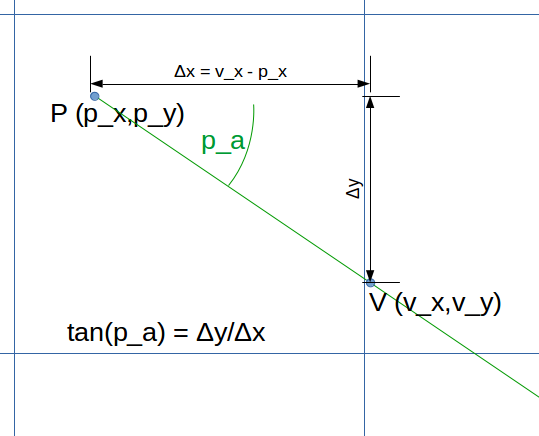
\includegraphics[width=8cm]{vcheck1.png} 
        \caption{Punkt V finden}
        \label{fig:vcheck1}
\end{figure}

$\Delta x$ ist ziemlich leicht zu berechnen: einfach $v\_x - p\_x$. Somit haben wir \[\tan a = \frac{-\Delta y}{v\_x - p\_x}\] oder \[\Delta y = -\tan a \cdot (v\_x - p\_x)\]. Also ist $v\_y = p\_y - \tan a \cdot (v\_x - p\_x)$. Nur in dem Spezialfall $a = \pi$ oder $a = 0$ ist $v\_y = p\_y$, da der Strahl sich nicht auf der y-Achse bewegt. Unser Code ist also:
\begin{Verbatim}[baselinestretch=1.0, xleftmargin=1cm]
if a == 0 or a == pi:
	v_y = p_y
else:
	v_y = int(p_y - math.tan(a)*(v_x-p_x))
\end{Verbatim}

\paragraph{Das Inkrement von Punkt V:}
Als n\"achstes m\"ussen wir herausfinden, wie viel nach links/rechts (\texttt{x\_i})und wie viel nach oben/unten (\texttt{y\_i}) wir gehen m\"ussen, um den neuen Punkt zu finden. Diese Werte werden f\"ur jede Iteration der Schleife zu den alten Koordinaten addiert. Weil wir immer auf der n\"achsten Vertikalen \"uberpr\"ufen, ist \texttt{x\_i} +/- \texttt{TILE}. Wie bei \texttt{v\_x} ist \texttt{x\_i} positiv, wenn der Strahl nach rechts verl\"auft, und sonst negativ. Da wir das schon f\"ur \texttt{v\_x} \"uberpr\"ufen, k\"onnen wir den Code in den gleichen \texttt{if}-Block stellen, um dies zu erlangen:
\begin{Verbatim}[baselinestretch=1.0, xleftmargin=1cm]
if (a < 0.5 * pi) or (a > 1.5 * pi):
	x_i = TILE
	v_x = (p_x // TILE)*TILE + TILE
else:
	x_i = -1 * TILE
	v_x = (p_x // TILE)*TILE - 1
\end{Verbatim}

\begin{figure}[htbp] 
        \centering
        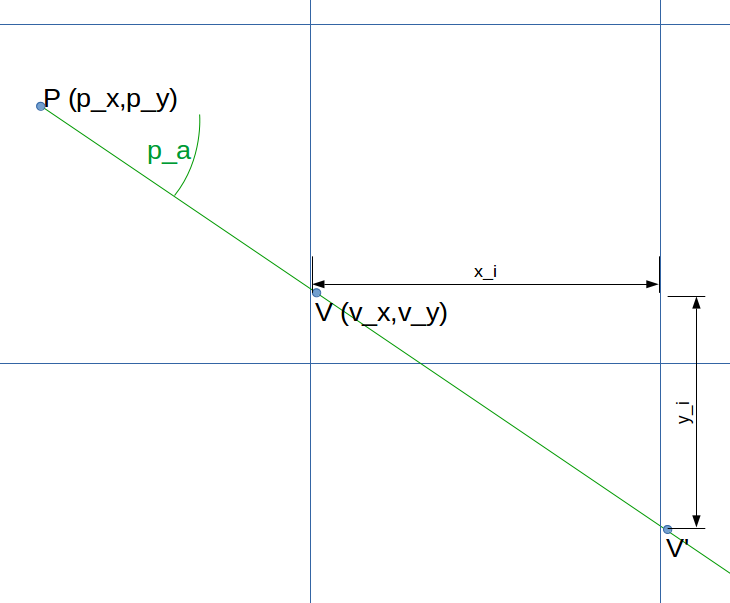
\includegraphics[width=8cm]{vcheck2.png} 
        \caption{x\_i und y\_i}
\end{figure}
Danach kommt y\_i, wozu wir wieder den Tangens brauchen. Dieses Mal ist es aber ein bisschen einfacher: Wieder haben wir \[\tan a = \frac{-y\_i}{x\_i}\]aber dieses mal Kennen wir schon \texttt{x\_i}, also formen wir einfach um zu \[y\_i = -\tan a \cdot x\_i\]
Auch hier ist $y\_i = 0$, wenn der Strahl horizontal ist. Eigentlich m\"ussen wir nicht einen zus\"atzlichen \texttt{if}-Block daf\"ur haben, denn $\tan 0 = 0$ und $\tan \pi = 0$, aber es hilft, dar\"uber bewusst zu sein. Jetzt ist unser ganzer Code, um diese Werte zu bestimmen, wie folgt:
\begin{Verbatim}[baselinestretch=1.0, xleftmargin=1cm]
# Get x_i (+TILE if pointing right, -TILE if left).
# Get v_x (x coord of the first point).
if (a < 0.5 * pi) or (a > 1.5 * pi): # pointing right
        x_i = TILE
        v_x = (p_x // TILE)*TILE + TILE
else:
        x_i = -1 * TILE
        v_x = (p_x // TILE)*TILE - 1

# Get y_i, using tan.
# Get v_y, using magic.
if a == 0 or a == pi: # completely horizontal ray
        y_i = 0
        v_y = p_y
else:
        y_i = int(math.tan(a) * (-1) * x_i)
        v_y = int(p_y - math.tan(a)*(v_x-p_x))
\end{Verbatim}

Leser, die den Code gelesen haben, haben vielleicht gemerkt, dass bei \texttt{y\_i} und \texttt{v\_y} um den Ausdruck die \texttt{int()} Funktion benutzt wird. Die Koordinaten m\"ussen noch immer \texttt{int}s bleiben, aber python konvertiert in einem Versuch, hilfreich zu sein, \texttt{int}s automatisch in \texttt{float}s.

\paragraph{Die Schleife:}
Jetzt, wo wir die n\"otigen Werte haben, k\"onnen wir die Schleife beginnen, die durch die Punkte iteriert. In der Schleife pr\"ufen wir einfach, ob der Punkt $(v\_x,v\_y)$ in einem ``vollen'' Feld oder nicht steht. Wie vorher beschrieben, ist die Methode, um von Koordinaten zu \texttt{world}-Koordinaten zu kommen, einfach $\lfloor k \div TILE \rfloor$, in python \texttt{k // TILE}. \\
Die Überpr\"ufung, ob Punkt V auf einem vollen Feld steht, ist also einfach \texttt{world[v\_x // TILE][v\_y // TILE]}: die Zellen sind sowieso 1 oder 0. Wenn das also 1 ist, wird \texttt{vvalid} also auf \texttt{True} gesetzt, und die Schleife verlassen. \\
Weil es passieren kann, dass der erste Punkt V schon au\ss erhalb des Spielfeldes ist, ist diese ganze Überpr\"ufung in einem \texttt{try} gepackt. Wenn ein \texttt{IndexError} passiert, \texttt{break}ed es wieder die Schleife und geht weiter zu den horizontalen Überpr\"ufungen. \\
Ansonsten werden zu \texttt{v\_x} und \texttt{v\_y} \texttt{x\_i} bzw. \texttt{y\_i} addiert, und die Schleife fortgesetzt, solang V noch ein g\"ultiger Punkt ist. Der resultierende Code ist also:
\begin{Verbatim}[baselinestretch=1.0, xleftmargin=1cm]
# hl is the number of cells along the horizontal
for i in range(hl):
        try:
                if world[v_x // TILE][v_y // TILE]:
                        vvalid = True
                        break
        except IndexError:
                if debug:
                        print("v. error!", v_x,v_y, \
                        "\n Ray:", p_x, p_y, a)
                break
        v_x += x_i
        v_y += y_i
        if v_x >= (hl*TILE) or v_y >= (vl*TILE):
                break
\end{Verbatim}

Zuletzt wird noch die Distanz zwischen den Punkten P und V berechnet, mit dem Satz des Pythagoras:
\begin{Verbatim}[baselinestretch=1.0, xleftmargin=1cm]
vdist = math.sqrt((v_x-p_x)**2 + (v_y-p_y)**2)
\end{Verbatim}
Damit haben wir die erste vertikale Grenze, die der Strahl schneidet.

\subsubsection{Horizontale Schnitte}
F\"ur die horizontalen Schnittpunkte machen wir ungef\"ahr das Gleiche wie f\"ur vertikale, nur die Achsen sind vertauscht: \texttt{y\_i} ist hier +/- \texttt{TILE}, und \texttt{x\_i} muss mit Tangens berechnet werden. Das Meiste kann aber leicht von dem Vorigen \"ubertragen werden. Zuletzt werden wir eine m\"ogliche Distanz in \texttt{hdist} haben, wenn \texttt{havlid True} ist.

\subsubsection{Vergleich und \texttt{return}}
Jetzt haben wir also minimal 0 Distanzen, und maximal 2. Mit einer einfachen \texttt{if} / \texttt{elif} Kette k\"onnen wir daraus die niedrigste Distanz finden: dann haben wir den ersten Punkt, an dem der Strahl auf etwas trifft. \\
Zuerst sehen wir, ob beide Werte \texttt{True} sind. Wenn schon, geben wir die k\"urzere Distanz zur\"uck:
\begin{Verbatim}[baselinestretch=1.0, xleftmargin=1cm]
if vvalid and hvalid: # both rays collide
        return min(vdist, hdist)
\end{Verbatim}
Danach wird einzeln gepr\"uft, ob \texttt{vvalid} bzw. \texttt{hvalid} Wahr sind. Entsprechend wird dann \texttt{vdist} oder \texttt{hdist} zur\"uckgegeben:
\begin{Verbatim}[baselinestretch=1.0, xleftmargin=1cm]
elif vvalid: # only vertical collision
        return vdist
elif hvalid:
        return hdist
\end{Verbatim}
Schlie\ss lich wird -1 zur\"uckgegeben, wenn der Strahl auf nichts trifft:
\begin{Verbatim}[baselinestretch=1.0, xleftmargin=1cm]
else: # no collision
        return -1
\end{Verbatim}

\begingroup
\renewcommand{\cleardoublepage}{}
\renewcommand{\clearpage}{}

\mychapter{3}{Schlussteil}
Jetzt habe ich hoffentlich verst\"andlich erkl\"art, wie genau ein Raycaster funktioniert. Das Prinzip ist ziemlich einfach, und ein gut geschriebener Raycaster braucht wenig Rechenleistung, auch wenn das Spielfeld sehr limitiert wird.

Die goldene Zeit des Raycaster war nicht sehr lang, aber produzierte Hits wie Wolfenstein 3D. Noch dazu wird das grundlegende Prinzip, den Weg eines Strahls zu verfolgen, noch immer in Raytracern benutzt.

Mein selbst geschriebener Raycaster ist nicht besonders schnell (was zum Teil auch an python liegt) und die Steuerung k\"onnte besser sein, aber sonst bin ich damit sehr zufrieden. Auch will ich die python Dokumentation und das \LaTeX\ Buch von WikiBooks loben, ohne die ich nicht sehr weit gekommen w\"are. Jetzt nur noch ein paar Quellen:
\endgroup

\begin{thebibliography}{9}

\bibitem{life}
  Gardner, Martin:
  \emph{ Mathematical Games – The fantastic combinations of John Conway's new solitaire game ``life''} --
  Scientific American 223 (link \url{http://ddi.cs.uni-potsdam.de/HyFISCH/Produzieren/lis_projekt/proj_gamelife/ConwayScientificAmerican.htm}),
  (10.1970)

\bibitem{permadi}
  Permadi, F.:
  \emph{Ray-Casting Tutorial For Game Development And Other Purposes} --
  \url{http://www.permadi.com/tutorial/raycast/}
  (1996)

\bibitem{pygamedocs}
  Pygame Team:
  \emph{Pygame Documentation} --
  \url{http://www.pygame.org/docs/}
  (Abgerufen 02.2015)

\bibitem{pythondocs}
  Python Software Foundation:
  \emph{Python 3.3 documentation} --
  \url{http://docs.python.org/3.3/}
  (Abgerufen 02.2015)

\bibitem{wolf3d}
  Sanglard, Fabien:
  \emph{Wolfenstein 3D For iPhone} -- 
  \url{http://www.fabiensanglard.net/wolf3d/index.php}
  (04.2009)

\bibitem{scratch}
  Scratch Wiki:
  \emph{Raycaster} --
  \url{http://wiki.scratch.mit.edu/w/index.php?title=Raycaster&oldid=105373},
  (06.09.2014)

\bibitem{latexbooks}
  Wiki Books:
  \emph{\LaTeX} --
  \url{http://en.wikibooks.org/w/index.php?title=LaTeX&oldid=2757849}
  (23.01.2015)

\bibitem{enwiki}
  Wikipedia:
  \emph{Ray casting} -- 
  \url{http://en.wikipedia.org/w/index.php?title=Ray_casting&oldid=639531500}
  (25.12.2014)

\bibitem{dewiki}
  Wikipedia:
  \emph{Raycasting} --
  \url{http://de.wikipedia.org/w/index.php?title=Raycasting&oldid=137530408},
  (07.01.2015)

\end{thebibliography}

\appendix

\chapter{Anhang 1: Hilfen zu \texttt{main.py}}
\section{Liste hilfreicher Variablen}
\begin{center}
	\begin{tabular}{|l|c|r|}
		\hline
		Variable & Datentyp & Beschreibung \\ \hline
		\hline
		\texttt{world} & 2-dim. Array & Das Spielfeld \\ \hline
		\texttt{TILE} & \texttt{int} & Gr\"o\ss e des \texttt{world}-Gitters \\ \hline
		\texttt{p\_x} & \texttt{int} & X-Koordinate des Spielers \\ \hline
		\texttt{p\_y} & \texttt{int} & Y-Koordinate des Spielers \\ \hline
		\texttt{p\_a} & \texttt{float} & Winkel des Spielers \\ \hline
		P & - & Punkt, an dem der Spieler steht (nur im Text) \\ \hline
		V & - & Punkt, an dem der Strahl eine Vertikale schneidet \\ \hline
		H & - & ditto, f\"ur die Horizontale \\ \hline
	\end{tabular}
\end{center}

\section{Struktur von \texttt{main.py}}
Um die Struktur des Programms zusammenzufassen:
\begin{spacing}{1.0}
\begin{framed}
\begin{enumerate}
	\item Diverse (globale) Variablen werden initialisiert
	\item Die zentrale Schleife des Spiels wird begonnen. Diese Schleife macht folgendes:
	\begin{itemize}
		\item Benutzereingaben holen, \texttt{walk()} oder \texttt{quit()} aufrufen
		\item Mit draw() rendern
		\item Mit update() die Welt aktualisieren
	\end{itemize}
\end{enumerate}
\end{framed}
\end{spacing}

\texttt{draw()} funktioniert so:
\begin{spacing}{1.0}
\begin{framed}
\begin{enumerate}
	\item Hintergrund malen
	\item Startwinkel bestimmen
	\item Durch die Spalten des Fensters iterieren:
	\begin{itemize}
		\item Strahl mit \texttt{cast()} werfen
		\item Mit der Distanz und \texttt{dist\_to\_offset()} Strich malen
		\item Winkel inkrementieren
	\end{itemize}
	\item Fenster aktualisieren
\end{enumerate}
\end{framed}
\end{spacing}

Und schlie\ss lich \texttt{cast()} selber:
\begin{spacing}{1.0}
\begin{framed}
\begin{enumerate}
	\item Auf Sonderf\"alle \"uberpr\"ufen
	\item Variablen initialisieren
	\item In einem \texttt{if}-Block nach vertikalen Schnittstellen pr\"ufen:
	\begin{itemize}
		\item Punkt V und Inkrement finden
		\item In einer \texttt{for}-Schleife den Strahl immer weiter f\"uhren:
		\begin{itemize}
			\item Pr\"ufen, ob V in einer lebenden Zelle ist
			\item V inkrementieren
		\end{itemize}
		\item Distanz berechnen
	\end{itemize}
	\item In noch einem \texttt{if}-Block nach horizontalen Schnittstellen pr\"ufen:
	\begin{itemize}
		\item Punkt H und Inkrement finden
		\item In einer \texttt{for}-Schleife den Strahl immer weiter f\"uhren:
		\begin{itemize}
			\item Pr\"ufen, ob H in einer lebenden Zelle ist
			\item H inkrementieren
		\end{itemize}
		\item Distanz berechnen
	\end{itemize}
	\item Distanzen vergleichen, Wert zur\"uckgeben
\end{enumerate}
\end{framed}
\end{spacing}

\chapter{Bilder}
\begin{figure}[htbp] 
        \centering
        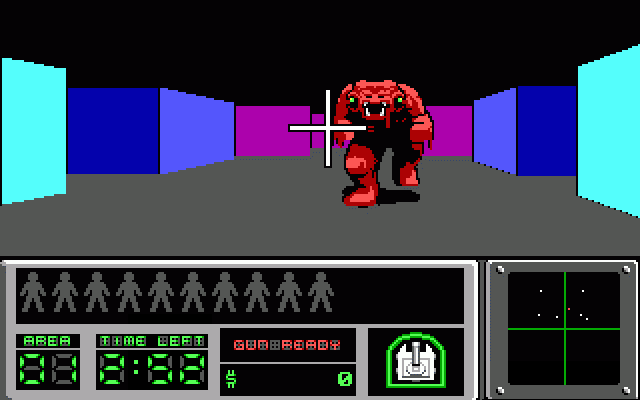
\includegraphics[width=10cm]{hovertank.png} 
		\caption{Hovertank 3D}
\end{figure}

\begin{figure}[htbp] 
        \centering
        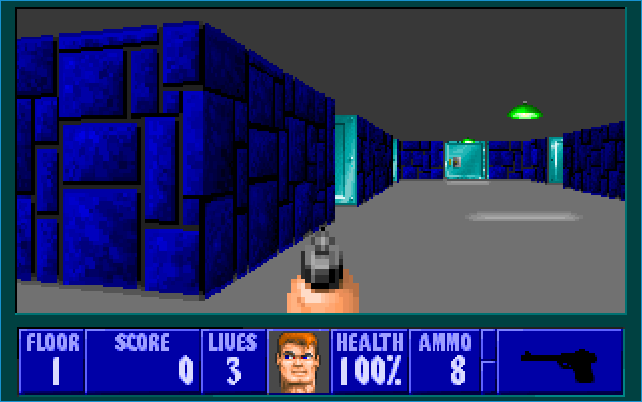
\includegraphics[width=10cm]{wolf3d.png} 
		\caption{Wolfenstein 3D}
\end{figure}

\end{document}
